\chapter*{Ejercicio 4}
\section*{Un balón de futbol americano}
En este ejercicio se trata de calcular aproximadamente el volumen V de un balón
de football americano profesional suponiendo que su superficie se genera rotando,
alrededor del eje horizontal, una curva y = y (x) que satisface que la longitud del eje
entre las dos puntas del balón es de 28 cm y la circunferencia de la máxima sección
circular transversal al eje mide 53 cm (véase la siguiente figura).

\begin{center}
    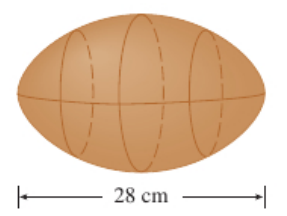
\includegraphics[height = 0.2\textheight]{recursos/Captura desde 2024-08-29 18-44-04.png}\par
\end{center}


a) Rebane la mitad derecha del balón en 10 cilindros de grosor $\Delta x = 1.4$ cm, de manera
que las rebanadas intersecten el eje x en los valores de la siguiente partición del intervalo
$[0, 14]$ 

1) Muestre que la parábola es, aproximadamente, la gráfica de la función
    $$y(x)=-0.043x^2 + 8.4352$$
definida para $-14\leq x\leq 14$


\begin{itemize}
    \item Sabemos que la $\text{Circunferencia}=2\pi r \therefore r=\frac{53}{2\pi}$
    \item La fórmula de las cónicas para la parábola es $y(x)=ax{^2}+bx+c$
    \item Sabemos que el radio de la circunferencia del balón es la longitud del radio cuando $x=0$, queremos saber el valor de y para $x=0$
\end{itemize}

\begin{gather*}
\therefore y(0)=\frac{53}{2\pi}=a(0){^2}+b(0)+c=c\\
\Rightarrow c=\frac{53}{2\pi}
\end{gather*}
También conocemos dos puntos que pasan por la ecuación del balón y son los puntos extremos, para encontrar los valores de $a,b$ sustituimos estos valores y resolvemos el sistema de ecuaciones
\begin{gather*}
y(14)=a(14){^2}+b(14)+c\\
y(-14)=a(-14){^2}+b(-14)+c\\
\text{-------------------------------------------------}\\
196a+c=0\\
+196a+c=0\\
\text{----------------------}\\
392a+2c\Rightarrow a=-\frac{2c}{392}=-\frac{c}{196}\\
\therefore y(x)=-\frac{c}{196}x{^2}+c\\
\Rightarrow y(x)=-\frac{\frac{53}{2\pi}}{196}x{^2}+\frac{53}{2\pi}\\
\end{gather*}
Simplificando tenemos que $$y(x)\simeq-0.0430x{^2}+8.4352$$
Podemos expresar la función en términos de $r_0$, de esta manera podemos deducir el dominio de la función.
\begin{gather*}
y(x)=-\frac{c}{196}x{^2}+c\\
y(x)=-\frac{r_{o}}{196}x{^2}+r_{o},\text{donde }r_o=c\\
\text{Igualamos a cero para determinar las raíces}\\
-\frac{r_{o}}{196}x{^2}+r_{o}=0\\
-\frac{r_{o}}{196}x{^2}=-r_{o}\\
-r_{0}x{^2}=-r_{0}(196)\\
x{^2}=\frac{-r_{0}(196)}{-r_{0}}\\
x=\pm \sqrt{196}\\
x=\pm 14\\
\therefore-14\leq x\leq 14
\end{gather*}
estos puntos, como habíamos definido antes, son los puntos de corte del centro del balón, solo estamos definiendo, en este caso la mitad de arriba del balón para aproximar su volumen. Esto de ve reflejado con el coeficiente $a$ negativo ($-a$).

2) Muestre que la aproximación del volumen (7) con los 10 cilindros circunscritos de grosor $\Delta x = 1.4 cm$ y radios $y(x_{k})$ cm para $k = 0, 1, 2, . . . , 9$ es:
$$V\simeq 2 \; x \;1825.5143=3651.0286 cm^3$$

La aproximación del volumen para el balón de futbol es: \begin{gather*}
    \sum_{k=0}^{9}V_{k}\\
    \text{donde: } V_{k}=\pi*r_{k}{^2}*\Delta h\\\Delta h=1.4,\text{la altura de cada cilindro}\\
    \end{gather*}
    el valor de correspondencia para cada $x_{k}=\Delta h*k$, la hayamos sustituyendo en la fórmula $r_{k}=y(x_{k})=y(x)\simeq-0.0430x_{k}{^2}+8.4352$.
Decimos que$$\sum_{k=0}^{9}V_{k}=\sum_{k=0}^{9}\pi*r_{k}{^2}\Delta h$$
Podemos decir que $\pi$ y $\Delta h$ son siempre constantes en la suma, por lo tanto podemos factorizar:

\begin{gather*}
=\pi \Delta h\sum_{k=0}^{9}r_{k}\\
=\pi \Delta h\sum_{k=0}^{9}(-0.0430x_{k}{^2}+8.4352){^2}
\end{gather*}

\begin{table}[!hbt]
    \begin{center}
    \begin{tabular}{| c | c | c | c | c | }
    \hline
    K & $\Delta h \cdot j$ & $y(x_{k})$ & $y(x_{k})^{2}$ & $\Delta h*\pi*y(x_{k}^2)$ \\ \hline
    0 & 0 & 8.4352 & 71.15259904 & 312.9462072 \\
    1 & 1.4 & 8.35092 & 69.73786485 & 306.7238667 \\
    2 & 2.8 & 8.09808 & 65.57889969 & 288.4317398 \\
    3 & 4.2 & 7.67668 & 58.93141582 & 259.1945103 \\
    4 & 5.6 & 7.08672 & 50.22160036 & 220.8866516 \\
    5 & 7 & 6.3282 & 40.04611524 & 176.1324259  \\
    6 & 8.4 & 5.40112 & 29.17209725 & 128.305885 \\
    7 & 9.8 & 4.30548 & 18.53715803 & 81.53086994  \\
    8 & 11.2 & 3.04128 & 9.249384038 & 40.68101085  \\
    9 & 12.6 & 1.60852 & 2.58733659 & 11.37972729  \\ \hline
\multicolumn{5}{ |r| } {suma $ = 1825.5143\;cm{^3}$}\\
\multicolumn{5}{|r|}{$V \simeq 2 x 1825.5143 = 3651.0286 cm3$}\\ \hline
    \end{tabular}
    \caption{Tabla de suma de los factores $x_k$}
    \label{tab:la suma de los cilindros circunscritos como parabola}
    \end{center}
    \end{table}

    Ya que solo calculamos los radios de la parte derecha del balón y considerando que es simétrico, el volumen de el lado derecho es el mismo que el del lado izquierdo, por lo tanto se multiplica por 2.
Muestre que la aproximación del volumen (7) con los 10 cilindros inscritos de
grosor $\Delta x = 1.4$ cm y radios $y (x_{k})$ cm para $k = 0, 1, . . . , 9$ es:
$$V\simeq 2 \; x \;1825.5143=3651.0286 cm^3$$
La aproximación del volumen para el balón de futbol es: 
\begin{gather*}
    \sum_{k=0}^{9}V_{k}\\
    \text{donde: } V_{k}=\pi*r_{k}{^2}*\Delta h\\\Delta h=1.4,\text{la altura de cada cilindro}\\
\end{gather*}
el valor de correspondencia para cada $x_{k}=\Delta h*k$, la hayamos sustituyendo en la fórmula $r_{k}=y(x_{k})=y(x)\simeq-0.0430x_{k}{^2}+8.4352$.
Decimos que$$\sum_{k=0}^{9}V_{k}=\sum_{k=0}^{9}\pi*r_{k}{^2}\Delta h$$
Podemos decir que $\pi$ y $\Delta h$ son siempre constantes en la suma, por lo tanto podemos factorizar:
\begin{gather*}
=\pi \Delta h\sum_{k=0}^{9}r_{k}\\
=\pi \Delta h\sum_{k=0}^{9}(-0.0430x_{k}{^2}+8.4352){^2}
\end{gather*}
\begin{table}[!hbt]
    \begin{center}
    \begin{tabular}{| c | c | c | c | c | }
    \hline
    K & $\Delta h \cdot j$ & $y(x_{k})$ & $y(x_{k})^{2}$ & $\Delta h*\pi*y(x_{k}^2)$ \\ \hline
    1 & 1.4 & 8.35092 & 69.73786485 & 306.7238667 \\
    2 & 2.8 & 8.09808 & 65.57889969 & 288.4317398 \\
    3 & 4.2 & 7.67668 & 58.93141582 & 259.1945103 \\
    4 & 5.6 & 7.08672 & 50.22160036 & 220.8866516 \\
    5 & 7   & 6.3282  & 40.04611524 & 176.1324259 \\
    6 & 8.4 & 5.40112 & 29.17209725 & 128.305885  \\
    7 & 9.8 & 4.30548 & 18.53715803 & 81.53086994 \\
    8 & 11.2& 3.04128 & 9.249384038 & 40.68101085 \\
    9 & 12.6& 1.60852 & 2.58733659  & 11.37972729 \\
   10 & 14  & 0.0072  & 5.184E-05   & 0.000228005 \\ \hline
\multicolumn{5}{ |r| } {suma $ = 1825.5143\;cm{^3}$}\\
\multicolumn{5}{|r|}{$V \simeq 2 x 1825.5143 = 3651.0286 cm3$}\\ \hline
    \end{tabular}
    \caption{Tabla de suma de los factores $x_k$}
    \label{tab:la suma de los cilindros inscritos}
    \end{center}
    \end{table}

    b) Suponga ahora que la curva $y = y (x)$ es la mitad superior de una elipse con
    centro en el origen, semieje horizontal $a = 14$ cm (sobre el eje x) y semieje vertical
    $$b = 53 2\pi \simeq 8.4352 cm (sobre el eje y).$$
    Partimos de la ecuación simétrica de la parábola.
    $$\frac{x{^2}}{a{^2}}+\frac{y{^2}}{b{^2}}=1$$Definimos los vértices en $v(0,14)$ y $v'(0,-14)$, por definición sabemos que la mitad de la longitud del semieje mayor es $a$, entonces a=14, $b$ es la mitad del semieje menor, el cual es el radio de nuestro balón, $\Rightarrow b=r_{0}=\frac{53}{2\pi}$
    $$\frac{x{^2}}{14{^2}}+\frac{y{^2}}{r_{0}{^2}}=1$$
    Reducimos hasta despejar a y.
    \begin{gather*}
    14{^2}r_{0}{^2}\left( \frac{x{^2}}{14{^2}} +\frac{y{^2}}{r_{0}{^2}}\right)= 1*14{^2}r_{0}{^2}\\
    \frac{14{^2}r_{0}{^2}x{^2}}{14{^2}} +\frac{r_{0}{^2}14{^2}y{^2}}{r_{0}{^2}}=14{^2}r_{0}{^2}\\
    r_{0}x{^2}+14{^2}y{^2}=14{^2}r_{0}{^2}\\
    14{^2}y{^2}=14{^2}r_{0}{^2}-r_{0}x{^2}\\
    y{^2}=\frac{14{^2}r_{0}{^2}-r_{0}x{^2}}{14{^2}}\\
    y{^2}=\frac{r_{0}{^2}}{14{^2}}(14{^2}-x{^2})\\
    y=\pm\sqrt{ \frac{r_{0}{^2}}{14{^2}}(14{^2}-x{^2}) }\\
    y=\frac{r_{0}}{14}*\pm\sqrt{(14{^2}-x{^2})}\\
    y=\frac{r_{0}}{14}*\pm\sqrt{196-x{^2}}
    \end{gather*}
    
    Sustituyendo $r_0=\frac{53}{2\pi}$ tenemos que $$\frac{r_{0}}{14}=\frac{\frac{53}{2\pi}}{14}\simeq 0.6025\therefore y(x)=0.6025\pm \sqrt{ 196-x{^2} }$$
    Podemos observar que $x{^2}$ solo puede valor, máximo 196 ya que la función no está definida para la raíz cuadrada de un número negativo. $\therefore -14\leq x\leq 14$ 
    
    d) Muestre que la aproximación del volumen (7) con los 10 cilindros circunscritos de
    grosor $\Delta x = 1.4 cm$ y radios $y (x_{k})$ cm para$k = 0, 1, 2, . . . , 9$ es:
    $$V \simeq 2 \times 2237.4593 = 4474.9186 cm3$$
    
    Partimos de que 
    $$V_{total}=\sum_{k=0}^{9}V_{k}$$
    donde $V_{k}=$ a cada volumen de disco con índice k y el volumen se traduce como$$V_{k}=\pi*\Delta h*r_{k}{^2}$$
    y el la medida del radio $r_{k}$ para cada cilindro circunscrito es el valor de $y(x_k)$, para $x_{k}=\Delta h*k$
    y $\Delta h$ es la altura correspondiente que es constante en cada cilindro.
    
    Así denotamos que \begin{gather*}
    \sum_{k=0}^{9}V_{k}=\sum_{k=0}^{9}\pi* r_{k}{^2}*\Delta h
    \end{gather*}
    donde $\pi$ y $\Delta h$ son siempre constantes, factorizamos
    \begin{gather*}
    \sum_{k=0}^{9}\pi* r_{k}{^2}*\Delta h
    =\pi \Delta h\sum_{k=0}^{9} r_{k}{^2}\\
    \text{sustituyendo }r_k \text{ por } y(x_{k})\\
    V_{total}=\pi \Delta h\sum_{k=0}^{9} y(x_{k}){^2}\\
    =\pi \Delta h\sum_{k=0}^{9} (0.6025 \sqrt{ 196-x_{k}{^2} }){^2}\\
    \end{gather*}
    así conseguimos la suma de los triangulo circunscritos para calcular el Balón de futbol.

    \begin{table}[!hbt]
        \begin{center}
        \begin{tabular}{| c | c | c | c | c | }
        \hline
        K & $\Delta h \cdot j$ & $y(x_{k})$ & $y(x_{k})^{2}$ & $\Delta h*\pi*y(x_{k})^2$ \\ \hline
        0 & 0    & 8.435       & 71.149225  & 312.930636 \\
        1 & 1.4  & 8.39271903  & 70.4377328 & 309.801329  \\
        2 & 2.8  & 8.26457839  & 68.303256  & 300.41341   \\
        3 & 4.2  & 8.04647716  & 64.7457948 & 284.766878  \\
        4 & 5.6  & 7.7308052   & 59.765349  & 262.861734  \\
        5 & 7    & 7.30492428  & 53.3619188 & 234.697977 \\
        6 & 8.4  & 6.748       & 45.535504  & 200.275607  \\
        7 & 9.8  & 6.02379488  & 36.2861048 & 159.594624   \\
        8 & 11.2 & 5.061       & 25.613721  & 112.655029   \\
        9 & 12.6 & 3.67673126  & 13.5183528 & 59.4568208   \\ \hline
    \multicolumn{5}{ |r| } {suma $2237.45404\; cm^3$}\\ \hline
        \end{tabular}
        \caption{Tabla de suma de los factores $x_k$}
        \label{tab:la suma de los cilindros circunscritos interpretados como una elipse}
        \end{center}
        \end{table}
        Como calculamos la mitad del balón, la suma de la parte derecha la multiplicamos por 2
$$\therefore V \simeq 2 \times 2237.4540 = 4474.90809 \;cm3$$
a) Muestre que la aproximación del volumen (7) con los 10 cilindros inscritos de
grosor $\Delta x = 1.4 cm$ y radios $y (xk)$ cm para$k = 1, 2, . . . , 10$ es:
$$V \simeq 2 \Delta 1924.5279 = 3849.0558 cm^3$$
Tenemos  la misma primicia del anterior.
$$V\simeq\pi \Delta h\sum_{k=1}^{10} (0.6025 \sqrt{ 196-x_{k}{^2} }){^2}$$

\begin{table}[!hbt]
    \begin{center}
    \begin{tabular}{| c | c | c | c | c | }
    \hline
    K & $\Delta h \cdot j$ & $y(x_{k})$ & $y(x_{k})^{2}$ & $\Delta h*\pi*y(x_{k})^2$ \\ \hline
    1 & 1.4  &  8.39271903 & 70.4377328 & 309.801329 \\
    2 & 2.8  &  8.26457839 & 68.303256  & 300.41341 \\
    3 & 4.2  &  8.04647716 & 64.7457948 & 284.766878 \\
    4 & 5.6  &  7.7308052  & 59.765349  & 262.861734 \\
    5 & 7    &  7.30492428 & 53.3619188 & 234.697977 \\
    6 & 8.4  &  6.748      & 45.535504  & 200.275607 \\
    7 & 9.8  &  6.02379488 & 36.2861048 & 159.594624 \\
    8 & 11.2 &  5.061      & 25.613721  & 112.655029 \\
    9 & 12.6 &  3.67673126 & 13.5183528 & 59.4568208 \\
   10 & 14   & 0           & 0          & 0          \\ \hline
\multicolumn{5}{ |r| } {suma $1924.52341\; cm^3$}\\\hline
    \end{tabular}
    \caption{Tabla de suma de los factores $x_k$}
    \label{tab:la suma de los cilindros inscritos interpretados como una elipse}
    \end{center}
    \end{table}
    \break
    Como calculamos la mitad del balón, la suma de la parte derecha la multiplicamos por 2.
    $$\therefore V \simeq 2 \times 1924.5279 = 3849.04682 cm3$$
